\documentclass[a4paper,11pt, oneside]{book}
\usepackage[utf8]{inputenc}
\usepackage[francais]{babel}
\usepackage[T1]{fontenc}
\usepackage{graphicx}
\usepackage{float}
\usepackage{wrapfig}
\usepackage{setspace}
\usepackage{geometry}
\usepackage{hyperref}
\usepackage{multicol}
\usepackage{etoolbox}
\usepackage{color}
\usepackage[explicit,pagestyles]{titlesec}
\usepackage[absolute,overlay]{textpos}
\usepackage{fancyhdr}
\usepackage{fontspec}
\usepackage{eurosym}
\usepackage{titlesec}


% ====== CONFIG ========

%\setmainfont{Roboto Light}

%\setmainfont{Roboto Light}
%\setsansfont{Roboto}
%\setmonofont{Roboto}
%\newfontfamily\light{Roboto Slab Light}
\graphicspath{{img/}}
\setlength{\unitlength}{1mm}
\makeatletter

\definecolor{primary}{RGB}{44, 62, 80}


\titleformat{\chapter}[display]{\huge}{\thechapter \quad #1}{0pt}{}
\titlespacing{\chapter}{0pt}{0pt}{0pt}

\titleformat{\section}[display]{\LARGE}{}{0pt}{\thesection \quad #1}


\setlength{\TPHorizModule}{1mm}
\setlength{\TPVertModule}{1mm}
\def\sizeMedia{38}
\def\size{3.8cm}
\def\sizeMargin{0.2cm}
\def\margin{2}
\def\fixMargin{0}

\pagestyle{plain}

\author{Yann Prono, Quentin Tardivon}
\date{\today}

\def\school{TELECOM Nancy}
\def\schoolAddress{193 Avenue Paul Muller}
\def\schoolPostalCode{54602}
\def\schoolCity{Villers-lès-Nancy}
\def\schoolCodeAndCity{\schoolPostalCode, \schoolCity}
\def\schoolYear{2016 - 2017}

\def\appName{MyAdblock}
\def\widthImage{1}

\def\schoolYear{2016 - 2017}

% ====== END CONFIG ========


\begin{document}

	\begin{titlepage}
		\thispagestyle{empty}

{\color{primary}



\includegraphics[width=4.0cm]{img/school-logo.eps}
\hspace{9mm}

\includegraphics[width=4.0cm]{img/collegium-logo.eps}
\hspace{5mm}

\includegraphics[width=4.0cm]{img/university-logo.eps}

\vspace{0.5cm}

	\begin{center}


			{\color[rgb]{0.8,0.8,.8}\rule{\textwidth}{0.8pt}}
			\vspace{0.5cm}

			\baselineskip=3pt
			{\Huge \bfseries{\appName}}\\
			\vspace{0.2cm}
			{\huge \bfseries{Réseaux et systèmes avancées}}
			\vspace{0.5cm}

		{\color[rgb]{0.8,0.8,.8}\rule{\textwidth}{0.8pt}}
		\vspace{0.5cm}


		
\includegraphics[width=0.6\textwidth]{logo.png}

		\Large{Quentin Tardivon}\\
		\Large{Yann Prono}

		\vspace{1.5cm}
		\large{\schoolYear}
	\end{center}

}

	\end{titlepage}


	\newpage\newpage\null\thispagestyle{empty}
	\newpage
		\tableofcontents
		\thispagestyle{empty}


	\chapter{Introduction}
	\setcounter{page}{1}

		La publicité sur internet est un moyen simple de gagner de l'argent.
		Celles-ci sont intégrés au sein même du site web (vidéos, bannières publicitaires...). L'abondance de contenus publicitaires apportent
		cependant quelques désavantages: L'utilisateur peut être distrait par ces publicités, la lecture du site web est plus difficile
		étant donnée la quantité d'information et l'affichage de ces publicités demandent plus de bande passante
		ainsi que de ressources pour le navigateur web.Il existe cependant des logiciels permettant de supprimer
		ces publicités. Ces logiciels vont analyser le flux entrant et sortant du navigateur afin de filtrer le contenu publicitaire.\\

		\noindent Dans le cadre de ce projet, nous devons développer un proxy ayant la même fonctionnaalité qu'un bloqueur de publicités.
		Ce proxy sera programmé en langage C à l'aide des sockets vu durant les cours.


	\chapter{Analyse}

		Afin de comprendre comment il est possible de filtrer les publicités, il est nécéssaire de comprendre fonctionne un navigateur web.
		On dispose de :
		\begin{itemize}
			\item Un navigateur web (le choix a peu d'importance dans le cadre de ce projet)
			\item Wireshark, un logiciel permettant capturer les paquets entrants et sortants de la machine\\
		\end{itemize}
		\noindent L'analyse des échanges TCP et HTTP se fera sur le site
		\href{http://www.telecomnancy.univ-lorraine.fr}{http://www.telecomnancy.univ-lorraine.fr}.
		Le site \href{http://www.01net.com}{http://www.01net.com} quant à lui sera utilisé pour
		analyser et tester le filtrage de publicités (abondance de publicités et la communication avec ce site n'est pas chiffrée).

		\section{Analyse du site telecomnancy.univ-lorraine.fr}

		Lorsque l'on souhaite accéder au site \href{http://www.telecomnancy.univ-lorraine.fr}{http://www.telecomnancy.univ-lorraine.fr} (on suppose que l'on dispose de l'adresse
		IP du serveur), des requêtes TCP (12, 13 et 14) sont envoyés au serveur afin d'initialiser la phase de connexion
		Suite à cela, une requête HTTP (15) de type \textit{GET} est envoyée au serveur afin de le contenu HTML du site web. La réponse du serveur est
		obtenu au paquet 29. Le contenu HTML est alors affiché dans le navigateur:

		\begin{figure} [htbp]
			\centering
			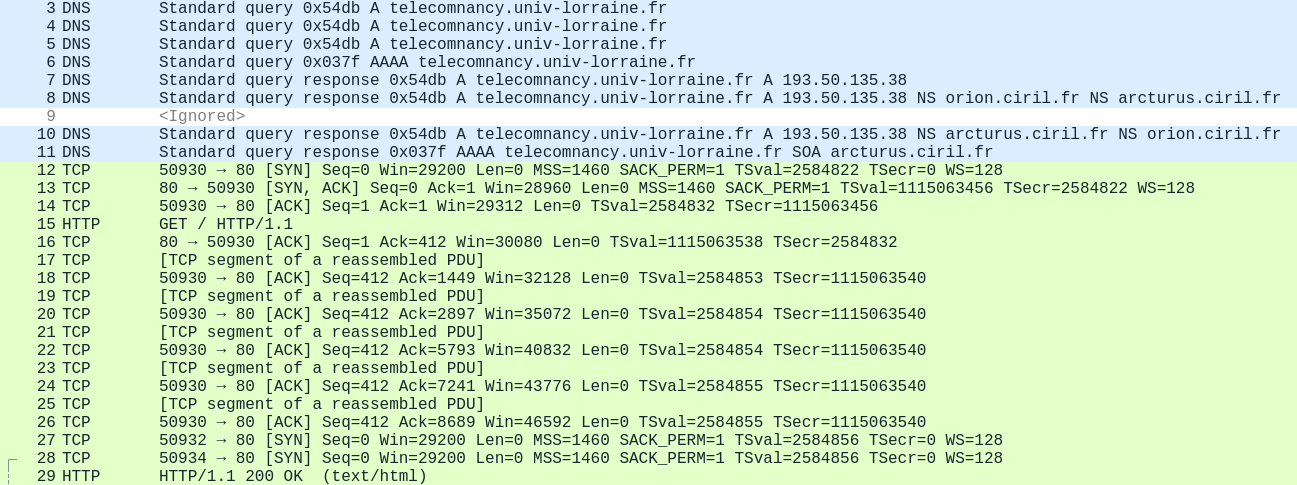
\includegraphics[width=\widthImage\textwidth]{1.png}\\
			\caption{Echanges de paquets au début de la communication}
		\end{figure}

		\noindent Cependant, le contenu HTML dépend d'autres ressources. Il est donc nécéssaire
		récupérer les différentes ressources (images, fichiers CSS, fichiers JS). De nouvelles requêtes sont alors envoyées (35, 38, 41...):

		\begin{figure} [htbp]
			\centering
			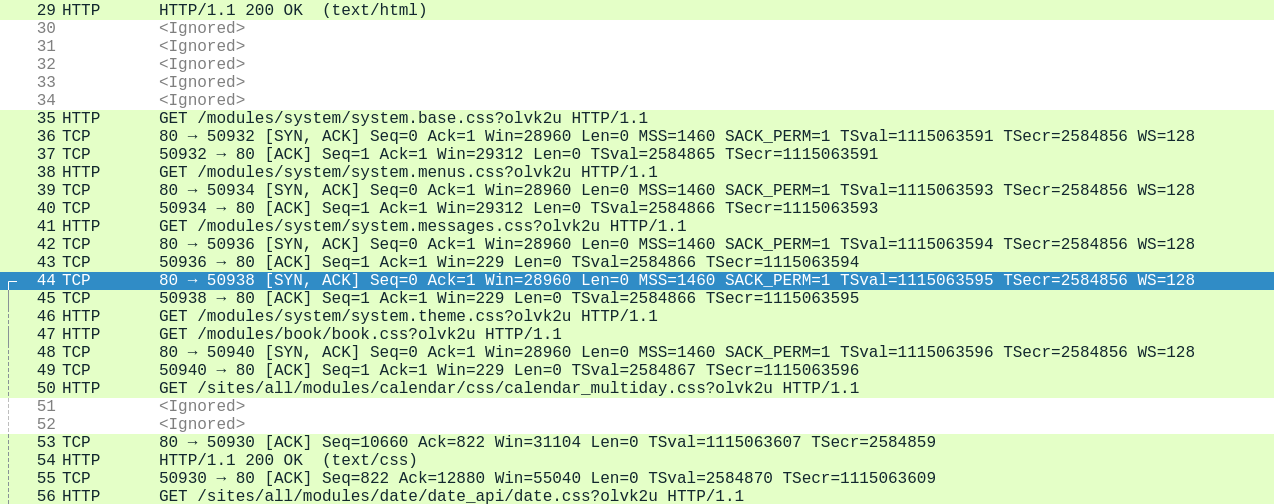
\includegraphics[width=\widthImage\textwidth]{2.png}\\
			\caption{Nouvelles requêtes émises suite à la réception du contenu HTML}
		\end{figure}


		On peut également retrouver l'ensemble de ces requêtes dans l'outil de développement integré dans les navigateurs web:

		\begin{figure} [htbp]
			\centering
			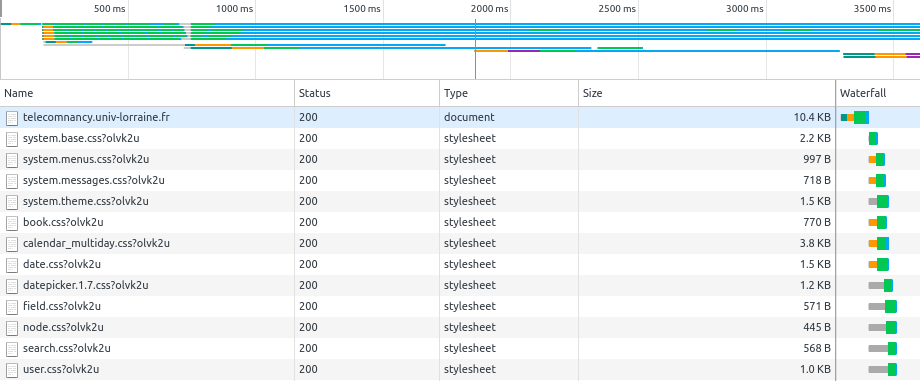
\includegraphics[width=\widthImage\textwidth]{3.png}\\
			\caption{Requêtes HTTP effectuées par le navigateur web}
		\end{figure}

\end{document}
